\documentclass[compress, xcolor=dvipsnames]{beamer}
\usepackage[utf8]{inputenc}
\usepackage{parskip}
\setlength{\parskip}{\medskipamount} 
\usepackage{tikz}
\tikzset{every picture/.style={line width=0.75pt}} %set default line width to 0.75pt 
 
\usepackage{caption}
\usepackage{subcaption}
\usepackage[nameinlink,capitalize]{cleveref}

  
\definecolor{navyblue}{rgb}{0.04706, 0.13725, 0.26667}
\definecolor{oxfordblue}{rgb}{0.0, 0.13, 0.28}
\definecolor{sapphire}{rgb}{0.03, 0.15, 0.4}

\usetheme{Berlin}
\usecolortheme[named=oxfordblue]{structure}
\usefonttheme[onlymath]{serif}
%\useoutertheme[footline=authortitle]{miniframes}

%gets rid of bottom navigation bars
%\setbeamertemplate{footline}[frame number]{}

%gets rid of bottom navigation symbols
\setbeamertemplate{navigation symbols}{}

%gets rid of footer
%will override 'frame number' instruction above
%comment out to revert to previous/default definitions
\setbeamertemplate{footline}{}

\addtobeamertemplate{navigation symbols}{}{%
    \usebeamerfont{footline}%
    \usebeamercolor[fg]{footline}%
    \hspace{1em}%
    \insertframenumber
}

% Vectors
\newcommand{\vect}[1]{\ensuremath{\textbf{#1}}}
\newcommand{\vecu}{\textbf{u}}
\newcommand{\grad}{\ensuremath{\nabla}}

% Misc
\newcommand{\deriv}[2]{\ensuremath{\frac{d #1}{d #2}}}
\newcommand{\pderiv}[2]{\ensuremath{\frac{\partial #1}{\partial #2}}}
\newcommand{\pderivtwo}[2]{\ensuremath{\frac{\partial^2 #1}{\partial #2^2}}}
\newcommand{\func}[2]{\ensuremath{#1\!\lrp{#2}}}
\renewcommand{\bar}[1]{\overline{#1}}

% Complexity
\newcommand{\bigo}[1]{\ensuremath{\operatorname{\mathcal{O}}\!\left(#1\right)}}
\newcommand{\bigomega}[1]{\ensuremath{\Omega\!\left(#1\right)}}

% Groups
\newcommand{\lrp}[1]{\left( #1 \right)}
\newcommand{\lrb}[1]{\left[ #1 \right]}
\newcommand{\lrc}[1]{\left\{ #1 \right\}}
\newcommand{\lrv}[1]{\left\langle #1 \right\rangle}
\newcommand{\abs}[1]{\left\lvert #1 \right\rvert}
\newcommand{\norm}[1]{\left\lVert #1 \right\rVert}

% Misc
\newcommand{\cexpz}{\ensuremath{e^{2k_i \lrp{x + \alpha_1 z}}}}
\newcommand{\cexpp}{\ensuremath{e^{2k_i \lrp{x + \alpha_1 \phi}}}}

\makeatletter
\setbeamertemplate{theorem begin}
{%
\begin{\inserttheoremblockenv}
{%
\inserttheoremname
\ifx\inserttheoremaddition\@empty\else\ \inserttheoremaddition\fi%
}%
}
\setbeamertemplate{theorem end}{\end{\inserttheoremblockenv}}
\makeatother

%------------------------------------------------------------
%This block of code defines the information to appear in the Title Page
\title{Modelling Surface Acoustic Wave Driven Flows over Topography}

\author{Bhargav Samineni}
%End of title page configuration block
%------------------------------------------------------------

\begin{document}
   
    \frame{\titlepage}    

    \section{Introduction}
    \begin{frame}
        Want to numerically simulate the flow of a fluid driven primarily by 
        high frequency surface acoustic waves over a surface that may include topography
        and may be inclined. 

        \begin{figure}[hb]
            \centering
            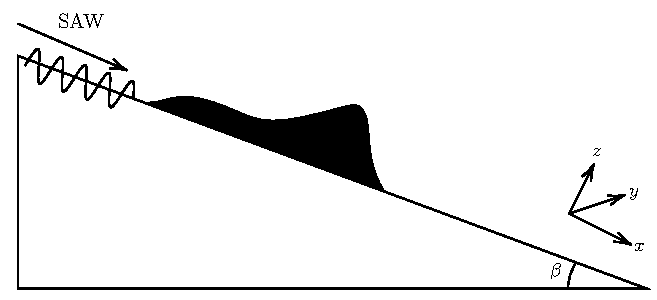
\includegraphics[width=.75\textwidth]{images/samp_diagram.pdf}
            \caption{A simplified sketch of a fluid flowing down an inclined plane with no topography.}
            \label{fig:model_diagram}
        \end{figure}
    \end{frame}
    \begin{frame}
        We let $\func{s}{x, y}$ describe the topography of the surface, 
        $\func{h}{x,y,t}$ be the film thickness relative to $\func{s}{x,y}$ at a time $t$, 
        and $\func{\phi}{x,y,t} = \func{s}{x,y} + \func{h}{x,y,t}$ be the height of the free surface at a time $t$.

        For completeness, we derive an equation to model fluids in a 
        3-D system, but we perform numerical simulations on the simplified 2-D case. 
    \end{frame}

    \section{Governing Equation}
    \subsection{Incompressible Navier-Stokes}
    \begin{frame}
        We start with the Incompressible Navier-Stokes Equation
        \begin{multline}
            \rho \lrp{\pderiv{\vecu}{t} + \lrp{\vecu \cdot \grad}\vecu} = -\grad p
            + \mu \grad^2 \vecu + \rho g \sin \beta \vect{i} - \rho g \cos \beta \vect{k} \\
            - \rho J e^{2k_i \lrp{x + \alpha_1 z}} \vect{i} - \rho J \alpha_1 e^{2k_i \lrp{x + \alpha_1 z}} \vect{k}
            \label{eq:ns-eq}
        \end{multline}
        where $\vect{u} =$ Fluid velocity, $p =$ Fluid pressure, $\rho =$ Fluid density, $\mu =$ Fluid viscosity, 
        $k_i =$  Attenuation coefficient, $\alpha_1 =$ Geometric constant, and $J = \lrp{1 + \alpha_1^2}A^2\omega^2 k_i$
        is a constant we define to consolidate terms. 

        The first two vector terms in the $x$ and $z$ direction represent the in plane and out of plane 
        components of gravity, while the last two vector terms represent the in plane and out of plane 
        components of the SAW forcing. 
    \end{frame}
    \subsection{Lubrication Approximation}
    \begin{frame}
        The Lubrication Approximation assumes we are dealing with thin films
        and allows us to ignore the inertial terms of the Navier-Stokes equation (LHS) as well as the in plane
        derivatives and normal component of $\vecu$. Hence, \cref{eq:ns-eq} reduces to 
        \begin{equation}
            \begin{aligned}
                \grad_2 p &= \mu \frac{\partial^2 \vect{v}}{\partial z^2} + \rho g \sin\beta \vect{i} - \rho J\cexpz\vect{i}\\
                \pderiv{p}{z} &= -\rho g \cos\beta - \rho J\alpha_1 \cexpz
            \end{aligned}
            \label{eq:lub_approx}
        \end{equation}
        where $\grad_2 = \lrp{\partial_x, \partial_y}$ and $\vect{v} = \lrp{u, v}$. 
    \end{frame}
    \subsection{Boundary Conditions}
    \begin{frame}

    \end{frame}

    \section{Numerical Simulation}
\subsection{Discretization}
\begin{frame}
    asdf
\end{frame}

\end{document}